\section{Spatial Regressions}
Looking at the regression analysis with the mean SIE we note that most of our fittings are not of great quality or statistically significant. We hope by introducing a spatial component to our analysis we can produce better quality results and begin to develop a more physical understanding of how these circulations impact the variability of sea ice in Antarctica.
Like before we start by doing individual regressions with each index we are interested in.
\begin{figure}[H]
    \centering
    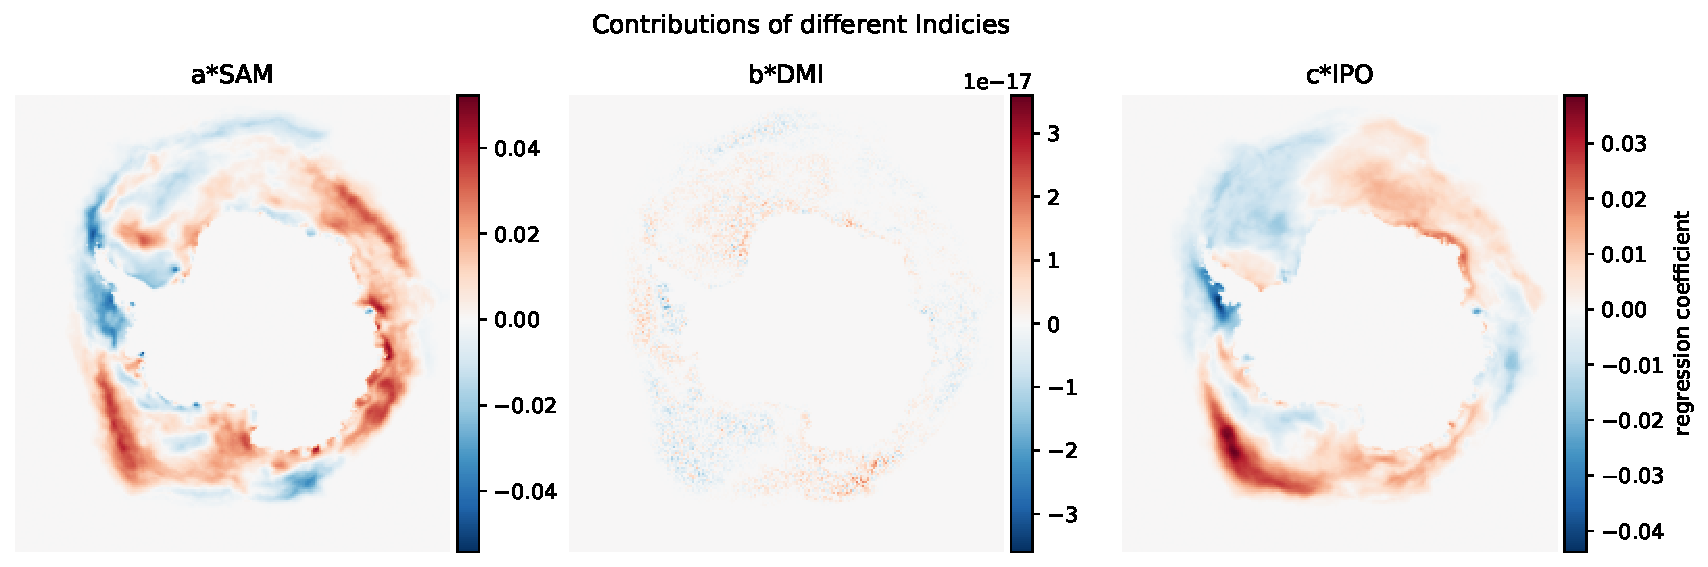
\includegraphics[width=\linewidth]{Images_3.0/regressions/index_contribution_anomalous_n1_annually_1979_2018.pdf}
    \caption[Spatial distribution of regression of SIC for each of the indices for 1979 to 2018]{Spatial distribution of regression of SIC for each of the indices for 1979 to 2018. Blue indicates a negative contribution and red indicates a positive contribution.}
    \label{fig:index_contribution_anomalous_n1_annually_1979_2018}
\end{figure}
Looking at these plots there are two main things which are notable. The first is that the expected contribution by DMI is much lower than the other two circulation patterns. For SAM this makes sense as it is localised around Antarctica. For IPO it also makes sense as the circulation is based over the Pacific \textcolor{red}{link this to the literature review.} The other thing to note is that the contribution of SAM and IPO are spatially very similar. This is interesting as we hypothesised that they impact the sea ice in Antarctica in different ways. It looking like SAM was more impactful for long term trends and IPO was more impactful for short term variability. This may or may not be the case. To understand this further we will need to look at the literature. As before this is done with a linear fitting, as such we don't expect the patterns here to indicate more that the base relationship that exists between these circulations and the behaviour of Sea ice in and around Antarctica. Likewise to before we will perform this same analysis, splitting the time series at the end of 2000, when IPO is noted to change it's overall phase. This can be seen below.

\begin{figure}[H]
    \begin{subfigure}{\linewidth}
    \centering
    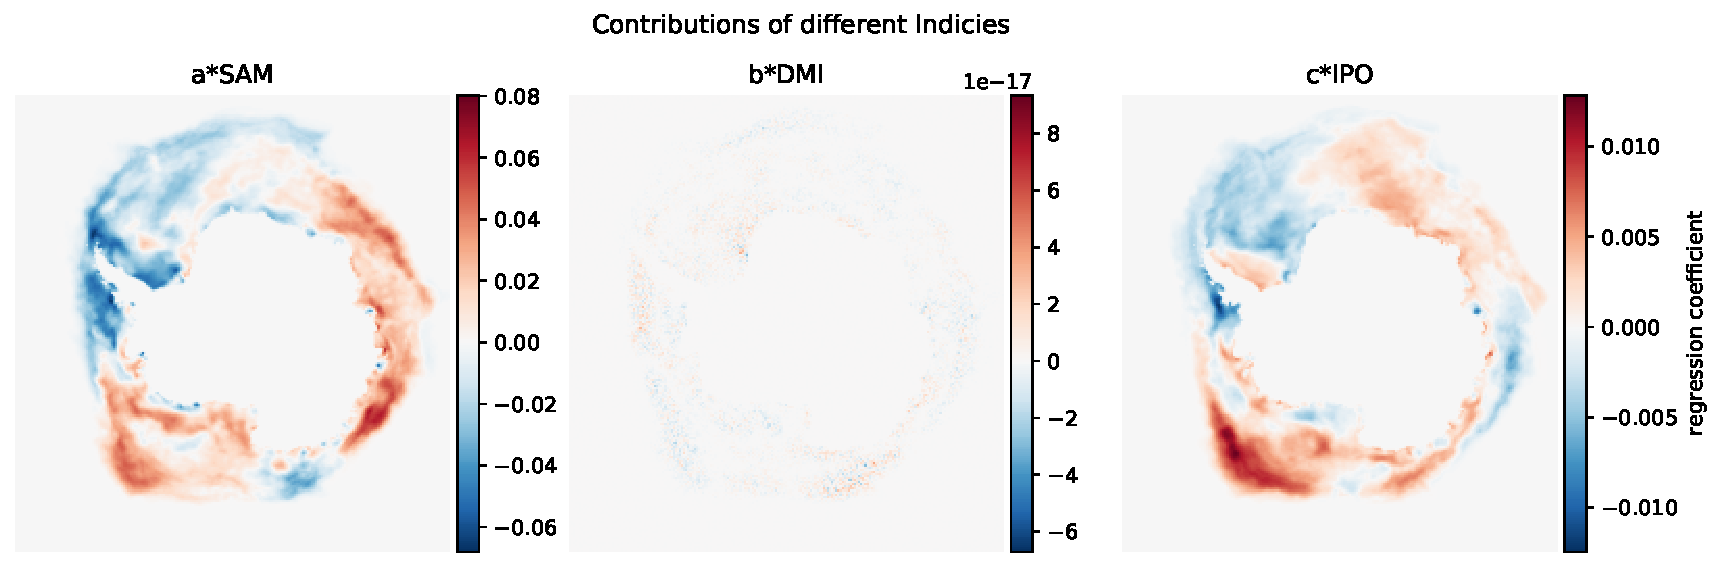
\includegraphics[width=\linewidth]{Images_3.0/regressions/index_contribution_anomalous_n1_annually_1979_2000.pdf}
    \caption{Spatial distribution of regression of SIC for each of the indices for 1979 to 2000.}
    \label{fig:index_contribution_anomalous_n1_annually_1979_2000}
    \end{subfigure}
    
    \begin{subfigure}{\linewidth}
    \centering
    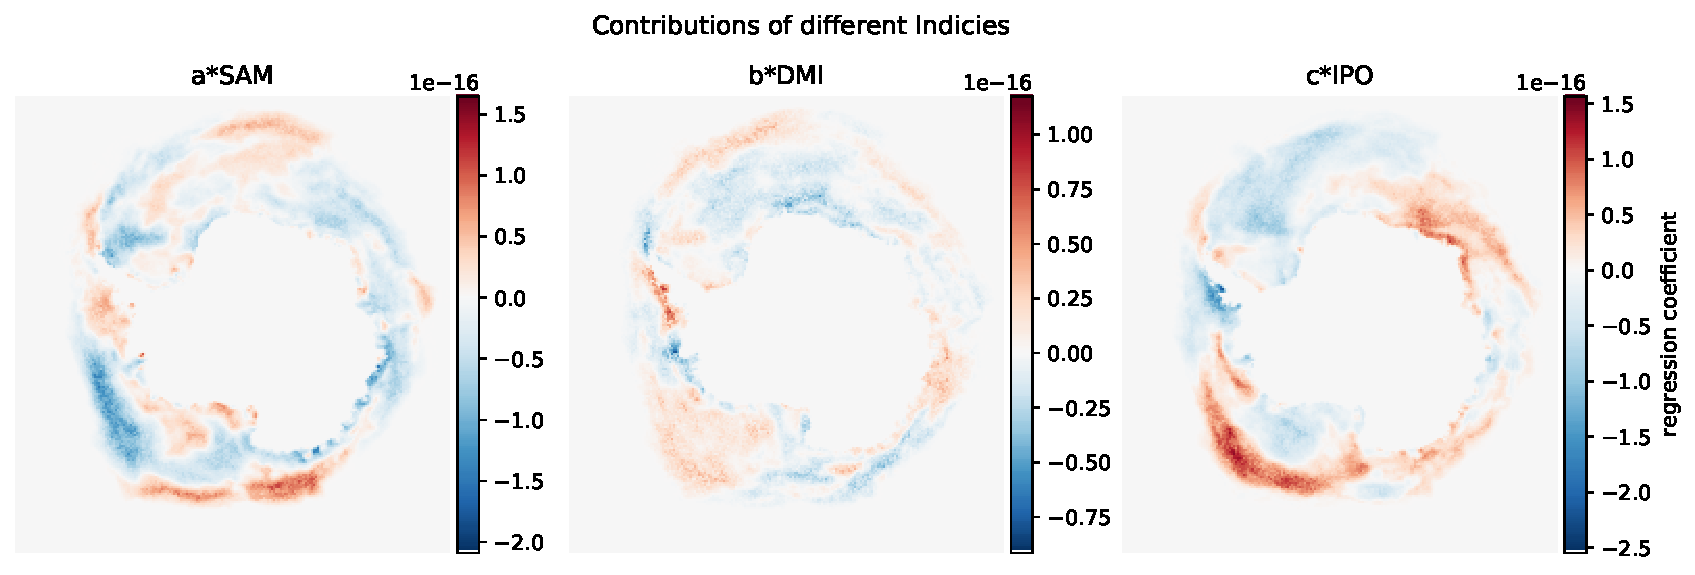
\includegraphics[width=\linewidth]{Images_3.0/regressions/index_contribution_anomalous_n1_annually_2001_2018.pdf}
    \caption{Spatial distribution of regression of SIC for each of the indices for 2001 to 2018.}
    \label{fig:index_contribution_anomalous_n1_annually_2001_2018}
    \end{subfigure}
    \caption{Spatial distribution of regressions for SIE for the different time periods in our dataset.}
\end{figure}